\documentclass{beamer}
\usetheme{Warsaw}
\useinnertheme{circles}
\useoutertheme[subsection=false]{smoothbars}
\usepackage[utf8x]{inputenc}
\usepackage[czech]{babel}
\usepackage[T1]{fontenc}
\usepackage{listings}
\usepackage{tikz}
\lstset{basicstyle=\tiny\ttfamily}
\logo{
\includegraphics[height=0.5cm]{brmlab.pdf}}

\begin{document}

\AtBeginSection[]
{
  \begin{frame}
    \frametitle{Outline}
    \tableofcontents[currentsection]
  \end{frame}
}

\title{brmiversity: Umělá inteligence \\ a teoretická informatika}
\subtitle{Přednáška č. 8}
\author{Petr Baudiš $\langle${\tt pasky@ucw.cz}$\rangle$}
\institute{
	brmlab 2011\\
	\vskip 1ex
	\pgfdeclareimage[height=4ex]{ccbysa}{by-sa.pdf}
	\pgfuseimage{ccbysa}
}
\date{}
\frame{\titlepage}

\section{Adaptivní agenti}

\subsection{}
\begin{frame}{Metody pro řízení agentů}
\begin{itemize}
\item Animat: Sensory --- umělá mysl --- efektory
\item Action selection problem
\vskip 3ex
\pause
\item Reaktivní if-then pravidla
\item Konečné stavové automaty
\item Free-flow architektura
\item Neuronové sítě (příště)
\item SOAR (později)
\end{itemize}
\end{frame}

\subsection{}
\begin{frame}[fragile]{Reaktivní plánování}
\begin{itemize}
\item {\bf Reaktivní plánování} vybírá pouze přímo následující akci na základě aktuálního kontextu
\vskip 3ex
\pause
\item If-then pravidla: {\bf If $p$ then $A$}, prioritizovaná \\ (``produkční pravidla'')
\item $A$ může být akce nebo sekvence akcí s pamětí (reflexy)
\item Rychlá evaluace: RETE a lazy vyhodnocování (později)
\end{itemize}
\hfill {\tiny (Brooks, 1986; Wooldridge, 2002)}
\begin{lstlisting}
# When starts: not at home && be in picking state
if see_obstacle then change_direction
if basketful_of_m. and picking then stop_picking
if see_mush. and picking then pick_up_the_mush.
if midday and picking then stop_picking
if home then END
if picking then move_random
if not_picking then move_home
\end{lstlisting}
\end{frame}

\subsection{}
\begin{frame}{Simple Hierarchical Reactive Planning}
\begin{itemize}
\item Dekomopzice? SHRP!
\item Hierarchické reaktivní plánování:
	$A$ může být sada dalších ifů --- podcíle,
	ifový strom s implicitním {\em and} po cestě
\item Modelový cyklus: \\ Appetitive $\to$ Taxis $\to$ Consumatory $\to$ Clean
\item Jak vybírat top-level cíle? Jízdní řád, pudy, dlouhodobé plány
\item Subsumpční architektura
\end{itemize}
\end{frame}

\subsection{}
\begin{frame}[fragile]{Parallel-rooted Ordered Slip-stack Hierarchy}
\begin{itemize}
\item POSH: Hierarchická if-then pravidla s pudy (drives), \\ postupy (competencies) a skripty (action patterns)
\item Drive: Základní reaktivní {\em patterny} okamžitě spouštějící reakce
\item Competency: Reaktivní {\em plány} postupně spouštějící reakce
\item Action pattern: Slepá posloupnost akcí
\end{itemize}

\hfill {\tiny (Bryson, 2002)}
\begin{lstlisting}
(RDC LIFE (GOAL (fail))
 (DRIVES
  ((grooming (TRIGGER ((want-to-groom))) groom-comp))
  ((receive-grooming (TRIGGER ((being-groomed))) tolerate-grooming))
  ((exploring (TRIGGER ()) explore-comp)))
 (C groom-comp (GOAL (fail)) (ELEMENTS
   ((groom-gp (TRIGGER ((partner-chosen) (aligned-w-target))) groom-note))
   ((new-partner-gp (TRIGGER ((being-groomed))) choose-groomer-as-partner))
   ((align-w-gp (TRIGGER ((partner-chosen) (touching-target))) engage))
   ((touch-gp (TRIGGER ((partner-chosen))) approach))
   ((choose-gp (TRIGGER ()) choose-grooming-partner))))
 (C explore-comp (GOAL (fail)) (ELEMENTS ...)))
\end{lstlisting}
\end{frame}

\subsection{}
\begin{frame}{Belief --- Desire --- Intention}
\begin{itemize}
\item Practical reasoning: Deliberative vs. means-ends
\item Obecná šablona výběru top-level cílů: BDI
\item Máme nějakou {\em představu}, na základě nich {\em toužíme} po různých věcech a z toho se dopracujeme k {\em úmyslu} něco konkrétního provést
\item Beliefs mohou být mylné
\item Desires jsou budoucí zajímavé možnosti agenta
\item Intentions jsou akce, ke kterým se agent rozhodl
\item Cyklus: Vygeneruj možnosti, rozhodni se pro jednu, \\ na základě vstupů profiltruj možnosti
\item Provádí se intentional stack, POSH-like
\end{itemize}
\end{frame}

\subsection{}
\begin{frame}{FSM a Fuzzy logika}
\begin{itemize}
\item Konečný automat; stav je akce (aktivuj efektor), \\ přechod je vstup (vstup ze senzorů)
\item Hierarchický FSM --- některé stavy jsou samy FSM; \\ umožňuje dekompozici
\item Probabilistický FSM --- přechody jsou asociovány i~s~pravděpodobnostmi
\vskip 3ex
\pause
\item Fuzzy množina $X$ je $(X,m)$, $m\colon X \to [0,1]$
\item Defuzzifikace --- weighted MOM
\item Fuzzy FSM --- fuzzy stavy i přechody, MIN-MAX metoda a~prahování stavů
\item Modelování emocí
\end{itemize}
\end{frame}

\subsection{}
\begin{frame}{Free-flow architektura}
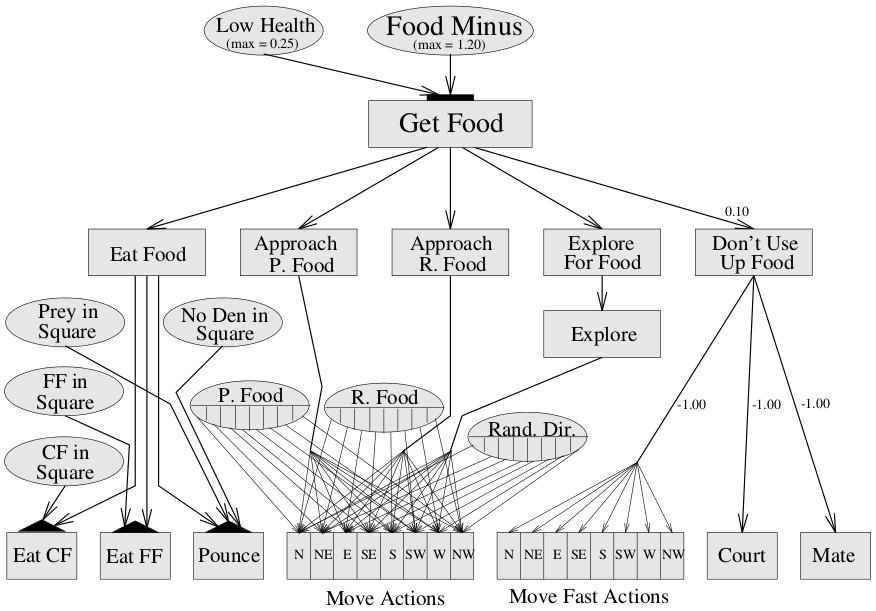
\includegraphics[width=9cm]{freeflow.png}
\hfill {\tiny (Tyrrell, 1993)}

Alternativy: Afordance; viz později reprezentace znalostí.
\end{frame}

\subsection{}
\begin{frame}{Otázky?}
\begin{center}
Příště: Metody pro učení agentů.
\end{center}
\end{frame}

\section{Neuronové sítě}

\subsection{}
\begin{frame}{ANN Revisited}
\begin{itemize}
\item Umělé neurony (``výpočetní krabičky'') \\ dostávají vstupy (čísla) a na jejich \\ základě generují výstup (číslo)
\item Obvykle: Vrstvy striktně oddělené, \\ vstupní vrstva se vstupy zvnějšku, \\ výstupní vrstva s výstupem pro uživatele, \\ skryté vrstvy vyhodnocují různé charakteristiky vstupů
\item Dnes: Více vrstev neuronů, jak je učit?
\end{itemize}
\begin{tikzpicture}[remember picture,overlay]
  \node [xshift=-4.5cm,yshift=-6cm,above right] at (current page.north east)
    {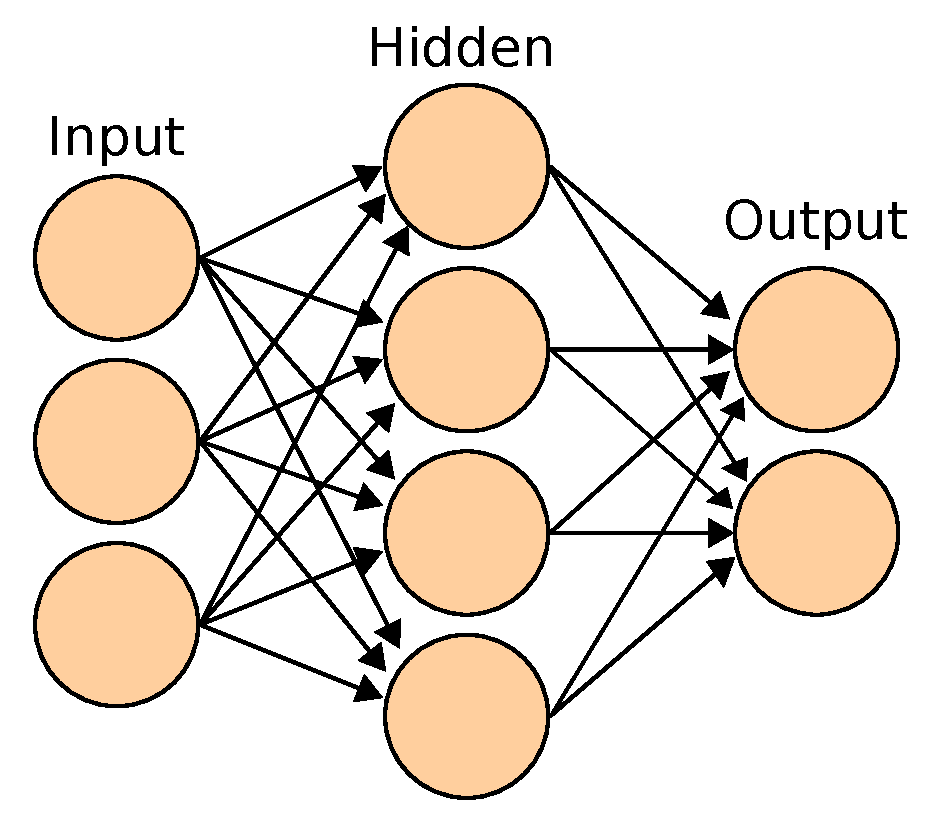
\includegraphics[width=4cm]{ANN.pdf}};
\end{tikzpicture}
\end{frame}

\subsection{}
\begin{frame}{Backpropagation Revisited}
\begin{itemize}
\item Myšlenka: Závislosti mezi vstupy a výstupy dokážeme přiměřeně matematicky popsat
\item Chceme upravit váhy podle {\em chyby}, kterou propagovaly; \\ větší váha nese větší chybu
\vskip 3ex
\pause
\item Iterujeme učení podle vstupních množin:
\begin{itemize}
\item Zjistíme chybu výstupu
\item Spočítáme {\em gradient} chyby podle vah jednotlivých spojů
\item Chybu se pokusíme zredukovat posunutím vah proti gradientu
\item Chybu ``zpětně šíříme'' do předchozí vrstvy a opakujeme
\end{itemize}
\end{itemize}
\end{frame}

\subsection{}
\begin{frame}{Vylepšení učení ANN}
\begin{itemize}
\item Inicializace vah: rozumně malé, náhodné, vyvážené
\item Chytřejší sestup podle gradientu
\item Rozšíření gradientu derivacemi druhého řádu
\item Relaxační metody: perturbace vah
\item Modulární sítě, úprava parametrů (prahy, neurony)
\item Genetické algoritmy
\end{itemize}
\end{frame}

\subsection{}
\begin{frame}{BP s momentem}
\begin{center}
Setrvačnost (moment): Zamez oscilacím v úzkých údolích \\
(zejména jsou-li osy různě dlouhé)

$$\Delta_E w_{i,j}(t+1) = -\alpha{\partial E \over \partial w_{i,j}(t)} + \gamma(w_{i,j}(t)-w_{i,j}(t-1))$$

Najít $\alpha$ a $\gamma$ je magie \\
$\alpha$ musí být kompromis mezi lokálními minimy a oscilacemi
\end{center}
\end{frame}

\subsection{}
\begin{frame}{Dynamický parametr učení}
\begin{center}
$$\Delta_E w_{i,j}(t+1) = -\alpha_i{\partial E \over \partial w_{i,j}(t)}$$

V nelineárním případě je třeba $\alpha_i$ volit dynamicky

\begin{block}{Silva-Almeida}
\begin{itemize}
\item {\bf Urychluj}, pokud se nezměnilo znaménko; $\alpha_i' = u\alpha_i$, $u > 1$
\item {\bf Zpomaluj}, pokud se znaménko změnilo; $\alpha_i' = d\alpha_i$, $d < 1$
\item Exponenciální růst/pokles může být příliš velký
\end{itemize}
\end{block}

\begin{block}{Delta-bar-delta}
\begin{itemize}
\item Pokud se nezměnilo znaménko; $\alpha_i' = u+\alpha_i$,
\item Pokud se znaménko změnilo; $\alpha_i' = d\alpha_i$, $d < 1$
\item Změna znaménka oproti $\delta_i' = (1-\Phi)\Delta_iE' + \Phi\delta_i$
\end{itemize}
\end{block}
\end{center}
\end{frame}

\subsection{}
\begin{frame}{Super SAB}
\begin{itemize}
\item Kombinace dynamického $\alpha$ a momentu
\item Zpětné šíření s momentem; pokud se nezměnilo \\ znaménko derivace, $\alpha_i' = \alpha^+\alpha_i$
\item Pokud se změnilo znaménko derivace, undo, \\ zmenši parametr učení $\alpha_i' = \alpha^-\alpha_i$ a zkus znovu
\end{itemize}
\end{frame}

\subsection{}
\begin{frame}{Interní reprezentace znalostí}
\begin{itemize}
\item Jak posoudit efektivitu interní reprezentace (vah skrytých neuronů)?
\vskip 3ex
\pause
\item Chceme neurony, které jsou aktivní (výstup 1), \\ pasivní (výstup 0) nebo tiché (0.5) \\
	``Něco mezi'' tolik nepřispívá k jednoznačné klasifikaci
\item Jak byste udělali vzoreček?
\vskip 3ex
\pause
\item TODO
\vskip 3ex
\pause
\item Ještě lepší je mít neurony, které jsou buď aktivní nebo pasivní (nejsou nikdy zbytečné)
\pause
\item Interní reprezentace by měla být jednoznačná \\ (hodně odlišná pro hodně odlišné výstupy)
\end{itemize}
\end{frame}

\subsection{}
\begin{frame}{Prořezávání ANN}
\begin{itemize}
\item Zbavíme se neuronů s uniformní reprezentací
\item Zbavíme se neuronů s identickou či inverzní reprezentací \\ vůči jiným
\item Výslednou síť nazveme {\em redukovanou}, můžeme ji vždy vytvořit
\end{itemize}
\end{frame}

\subsection{}
\begin{frame}{Otázky?}
\begin{center}
Příště: ANN úplně jinak --- asociativní paměti.
\end{center}
\end{frame}

\section{Vyčíslitelnost}

\subsection{}
\begin{frame}{Věta o rekurzi}
\begin{itemize}
\item Mějme ČRF $f$. Pak $\exists a$ (tzv. pevný bod), $\forall x: \Psi(f(a), x) \simeq \Psi(a, x)$
\item Důkaz: Mějme $a = s_1(z,z)$ ($z$ si vymyslíme).
	\\ $\Psi(s_1(z,z), x)$ má index $e$ a lze zapsat jako $\Psi(s_1(z,z),x) \simeq \Psi(e, z, x) \simeq \Psi(s_1(e, z), x)$. \\
	Můžeme dosadit $z=e$ a dostaneme $\Psi(f(a),x) \simeq \Psi(f(s_1(e,e)),x) \simeq \Psi(e, e, x) \simeq \Psi(s_1(e, e), x) \simeq \Psi(a, x)$.
\vskip 3ex
\item Varianty: Můžeme vyrobit místo $a$ celou funkci $g$ a~udělat to pro více proměnných.
\end{itemize}
\end{frame}

\subsection{}
\begin{frame}{Riceova věta}
\begin{itemize}
\item Mějme netriviální třídu ČRF $A$. Pak množina $B = \{x: \Psi(x) \in A\}$ není rekurzivní
\pause
\item Nelze určit, zda dva programy dělají to samé!
\vskip 3ex
\pause
\item Důkaz sporem: Vezměme $b \in B$ a $c \notin B$. \\
	Sestrojme $f(x)$, $f(B) = c$, $f(\bar B) = b$. \\
	Nalezněme pevný bod $e$. Co když $e \in B$ resp. $e \notin B$?
\end{itemize}
\end{frame}

\subsection{}
\begin{frame}{Otázky?}
\begin{center}
Příště: Algoritmicky nerozhodnutelné problémy.
\end{center}
\end{frame}

\subsection{}
\begin{frame}{Děkuji vám}
\begin{center}
{\bf pasky@ucw.cz}

\vskip 6ex

Příště: Umělá inteligence (strojové učení).
	Neuronové sítě. \\
	Evoluční algoritmy (schémata, EP, GP). \\
	Datové struktury (binární vyhledávací stromy).
\end{center}
\end{frame}

\end{document}
